\documentclass[11pt,]{article}
\usepackage[left=1in,top=1in,right=1in,bottom=1in]{geometry}
\newcommand*{\authorfont}{\fontfamily{phv}\selectfont}

\usepackage[]{mathpazo}


  \usepackage[T1]{fontenc}
  \usepackage[utf8]{inputenc}

\usepackage{abstract}
\renewcommand{\abstractname}{}    % clear the title
\renewcommand{\absnamepos}{empty} % originally center

\renewenvironment{abstract}
 {{%
    \setlength{\leftmargin}{0mm}
    \setlength{\rightmargin}{\leftmargin}%
  }%
  \relax}
 {\endlist}

\makeatletter
\def\@maketitle{%
  \newpage
%  \null
%  \vskip 2em%
%  \begin{center}%
  \let \footnote \thanks
    {\fontsize{18}{20}\selectfont\raggedright  \setlength{\parindent}{0pt} \@title \par}%
}
%\fi
\makeatother




\setcounter{secnumdepth}{0}


\usepackage{graphicx,grffile}
\makeatletter
\def\maxwidth{\ifdim\Gin@nat@width>\linewidth\linewidth\else\Gin@nat@width\fi}
\def\maxheight{\ifdim\Gin@nat@height>\textheight\textheight\else\Gin@nat@height\fi}
\makeatother
% Scale images if necessary, so that they will not overflow the page
% margins by default, and it is still possible to overwrite the defaults
% using explicit options in \includegraphics[width, height, ...]{}
\setkeys{Gin}{width=\maxwidth,height=\maxheight,keepaspectratio}

\title{Lab 3: Photosynthesis \thanks{\textbf{Current version}: February , 2019}  }



\author{\Large BIO 3103, Baylor University\vspace{0.05in} \newline\normalsize\emph{}  }


\date{}

\usepackage{titlesec}

\titleformat*{\section}{\Large\bfseries}
\titleformat*{\subsection}{\normalsize\itshape}
\titleformat*{\subsubsection}{\normalsize\itshape}
\titleformat*{\paragraph}{\normalsize\itshape}
\titleformat*{\subparagraph}{\normalsize\itshape}





\newtheorem{hypothesis}{Hypothesis}
\usepackage{setspace}

\makeatletter
\@ifpackageloaded{hyperref}{}{%
\ifxetex
  \PassOptionsToPackage{hyphens}{url}\usepackage[setpagesize=false, % page size defined by xetex
              unicode=false, % unicode breaks when used with xetex
              xetex]{hyperref}
\else
  \PassOptionsToPackage{hyphens}{url}\usepackage[unicode=true]{hyperref}
\fi
}

\@ifpackageloaded{color}{
    \PassOptionsToPackage{usenames,dvipsnames}{color}
}{%
    \usepackage[usenames,dvipsnames]{color}
}
\makeatother
\hypersetup{breaklinks=true,
            bookmarks=true,
            pdfauthor={BIO 3103, Baylor University ()},
             pdfkeywords = {},  
            pdftitle={Lab 3: Photosynthesis},
            colorlinks=true,
            citecolor=blue,
            urlcolor=blue,
            linkcolor=magenta,
            pdfborder={0 0 0}}
\urlstyle{same}  % don't use monospace font for urls

% set default figure placement to htbp
\makeatletter
\def\fps@figure{htbp}
\setlength{\intextsep}{25pt}  % sets space after text/before float figure
\makeatother

\usepackage{multicol}
\usepackage{textcomp}
\usepackage{textgreek}
\usepackage{pdflscape}
\usepackage{float}
\usepackage{booktabs}
\usepackage{makecell}
\usepackage[table]{xcolor}


% add tightlist ----------
\providecommand{\tightlist}{%
\setlength{\itemsep}{0pt}\setlength{\parskip}{0pt}}

\begin{document}
	
% \pagenumbering{arabic}% resets `page` counter to 1 
%


% \maketitle

{% \usefont{T1}{pnc}{m}{n}
\setlength{\parindent}{0pt}
\thispagestyle{plain}
{\fontsize{18}{20}\selectfont\raggedright 
\maketitle  % title \par  

}

{
   \vskip 13.5pt\relax \normalsize\fontsize{11}{12} 
\textbf{\authorfont BIO 3103, Baylor University} \hskip 15pt \emph{\small }   

}

}




\noindent  \hypertarget{background-information}{%
\section{Background information}\label{background-information}}

\newcommand{\textunderscript}[1]{$_{\text{#1}}$}

In the presence of light, photosynthetic organisms can utilize light and
carbon dioxide (CO\textsubscript{2}) to make sugars - the process of
photosynthesis. The sugars made are used by these organisms, and the
organisms that eat them, as a source of energy. A by-product of
photosynthesis is the liberation of oxygen (O\textsubscript{2}).

Alongside photosynthesis, these organisms are consuming oxygen via
respiration. Though respiration is always occuring, photosynthesis is a
light-dependent process and only occurs during certain hours of the day.
It is impossible to directly measure gross photosynthesis (or the total
amount of O\textsubscript{2} produced), but we \emph{can} measure
respiration (R) as the \textbf{rate of O\textsubscript{2} consumed} in
the dark, and the \textbf{rate of O\textsubscript{2} produced} in the
presence of light as a measure of net photosynthesis
(P\textsubscript{net}). Combining these direct measurements, we can
estimate gross photosynthesis (P\textsubscript{gross}).

\begin{equation}
\color{blue} P_{net} \color{black}= \color{red}P_{gross} \color{black}- \color{blue}R
\end{equation}

Using the equation above, we can direclty measured terms in \color{blue}
blue \color{black}, and may use them to calculate \color{red}
P\textsubscript{gross} \color{black}.

Organisms capable of photosynthesis span an incredible range of
morphology, from \emph{unicellular algae} to \emph{vascular plants}
(Fig. @ref(fig:organisms)). While every algae cell is photosynthetic,
\emph{aquatic macrophytes} (i.e.~vascular plants adapted to live in
aquatic ecosystems) have large amounts of specialized tissue devoted to
the transportation of resources and structural support. These two
organisms compete for very similar resources (such as sunlight and
dissolved nutrients) - how do their morphological adaptations convey a
competitive advantage?

\begin{figure}
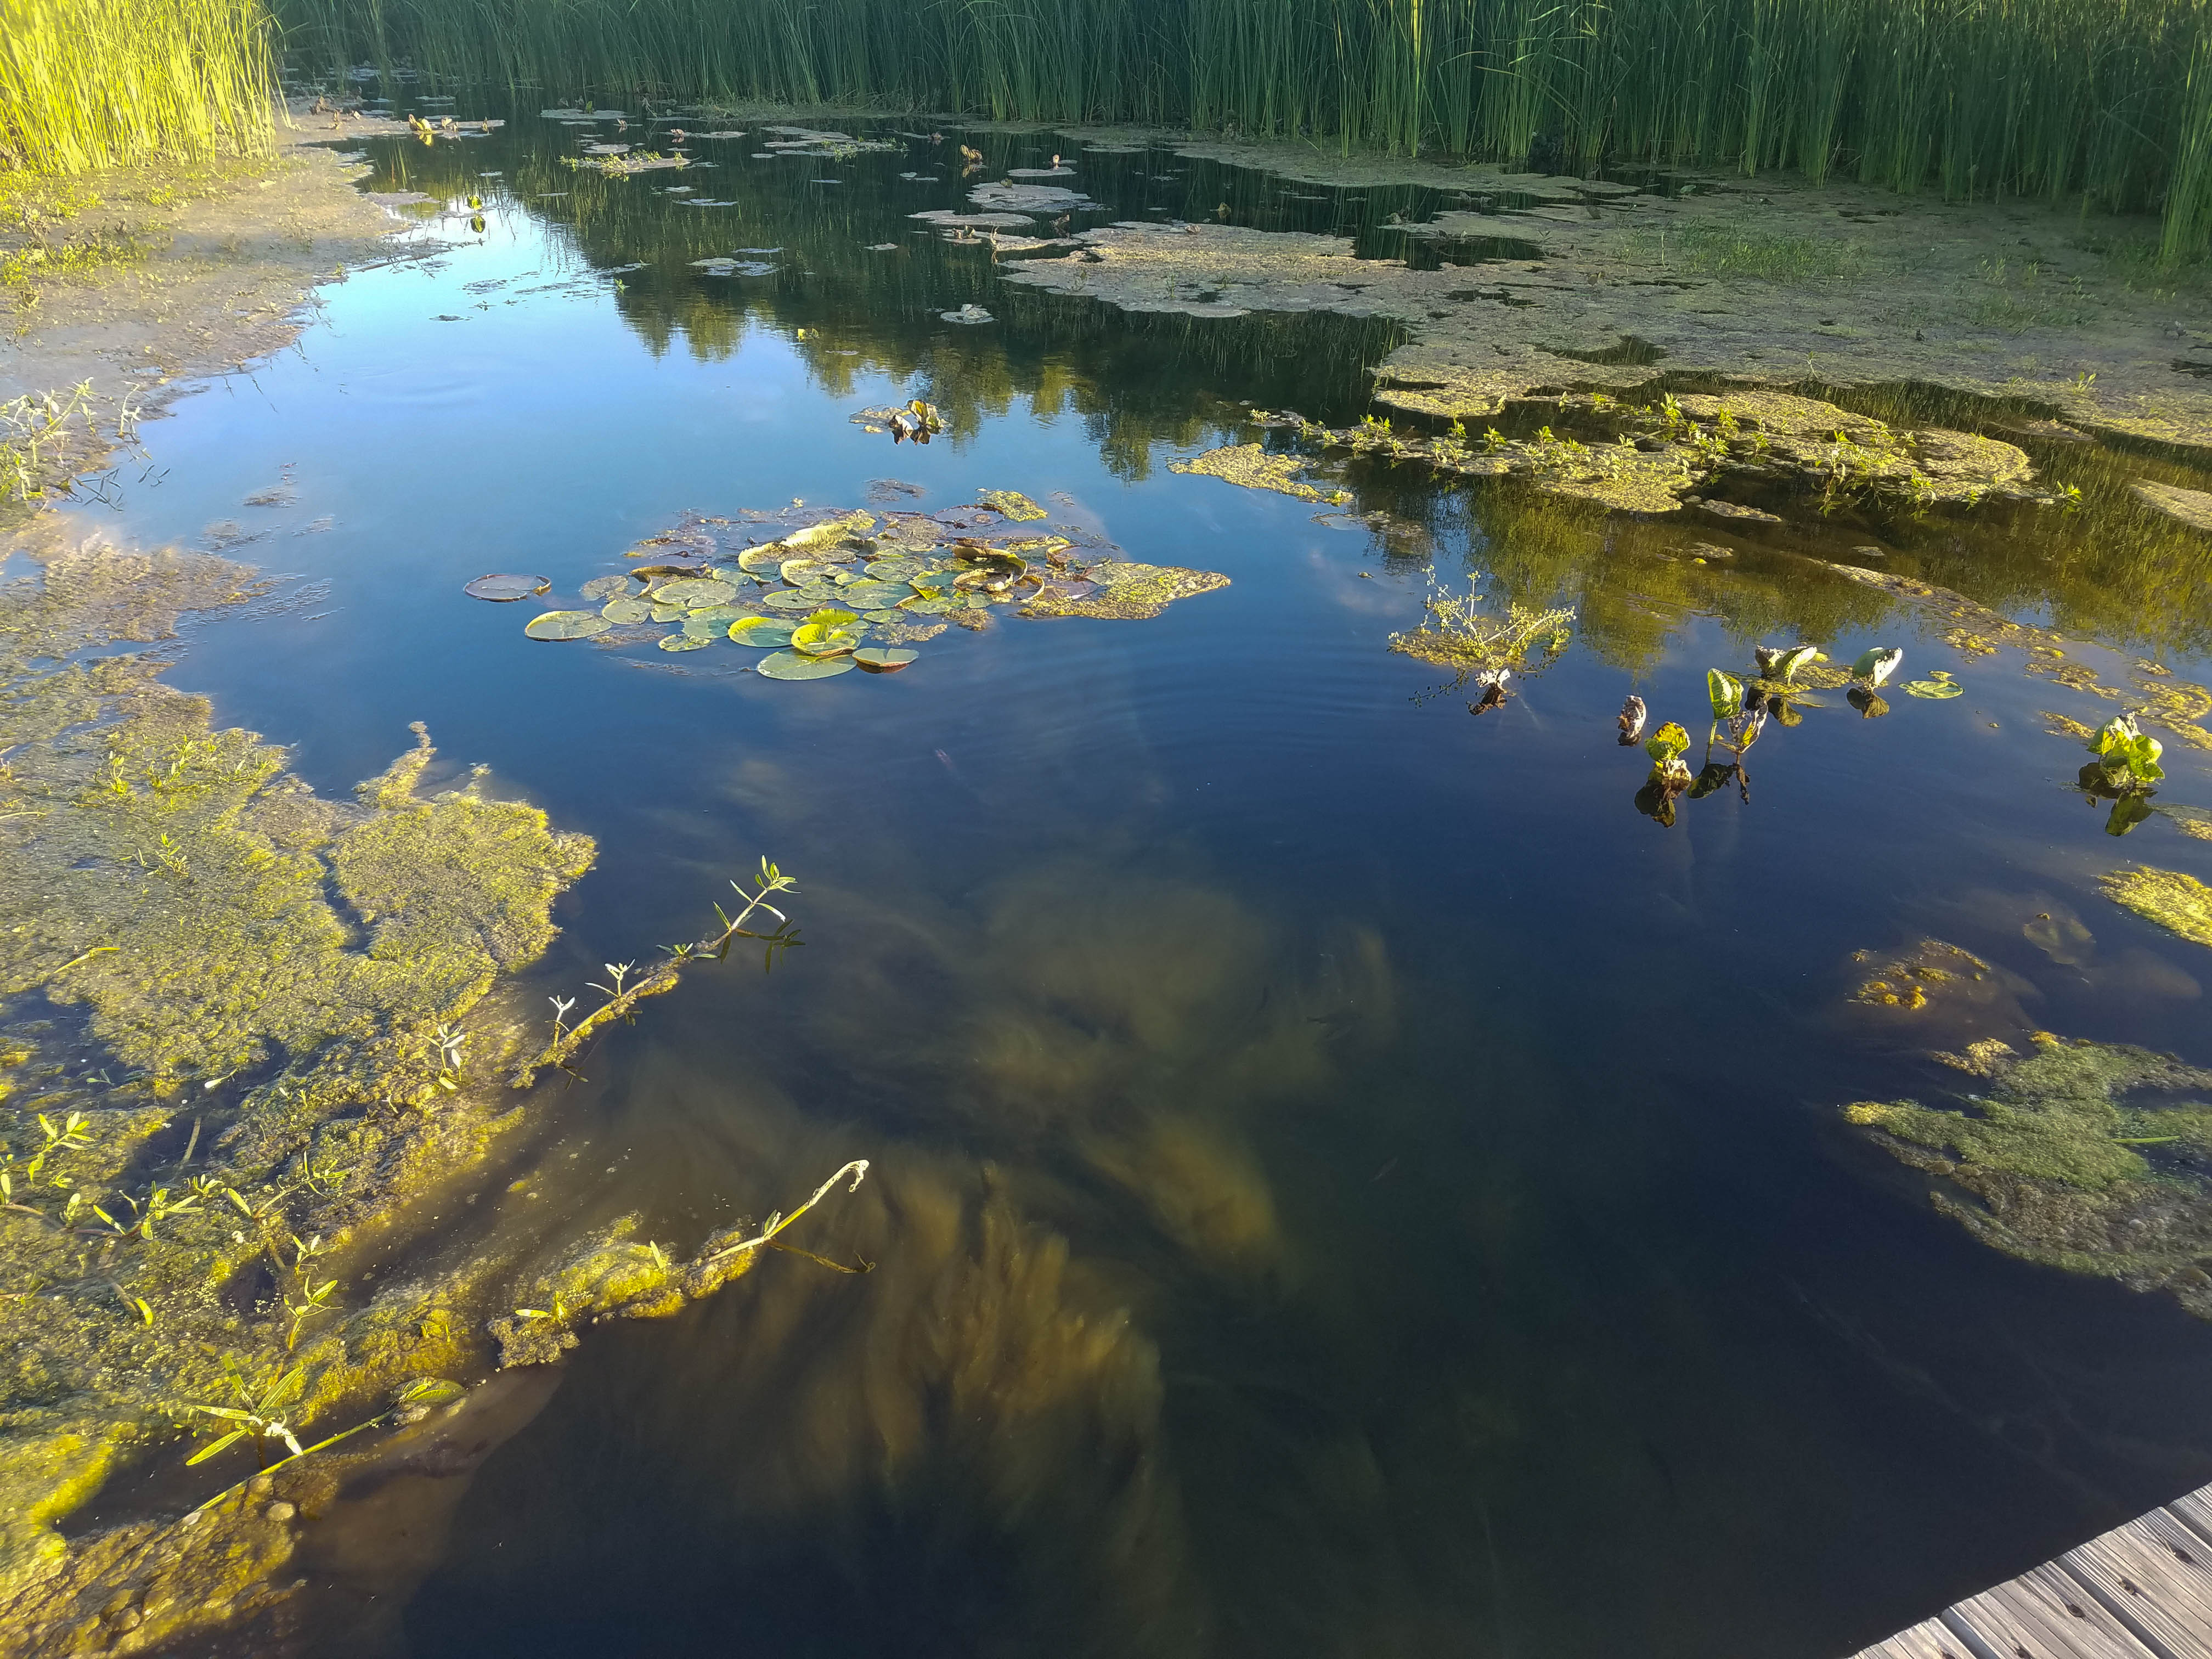
\includegraphics[width=0.5\linewidth]{../_chapter_materials/aquatic_photosynthesis} \includegraphics[width=0.5\linewidth]{../_chapter_materials/ludwigia} \caption{Aquatic algae (left pane, in both meta- and periphyton communities) and aquatic macrophytes (right pane) are photosynthetic organisms that evolved in aquatic ecosystems.}\label{fig:organisms}
\end{figure}

\hypertarget{objectives}{%
\section{Objectives}\label{objectives}}

You will form hypotheses to test questions about photosynthesis in 2
aquatic organisms - algae and a common aquatic macrophyte.

\begin{enumerate}
\def\labelenumi{\arabic{enumi}.}
\item
  Which organism has the highest rate of \emph{biomass specific} gross
  photosynthesis?
\item
  Which organism has the highest rate of \emph{biomass-specific}
  respiration?
\item
  Which organism has the highest rate of net primary production (NPP)
  per day?
\end{enumerate}

\bigskip

\pagebreak

\hypertarget{materials-methods}{%
\section{Materials \& methods}\label{materials-methods}}

You will be using a common \textbf{oxygen-change method} to determine
rates of photosynthesis and respiration. Biological oxygen demand (BOD)
bottles use a stopper that prevents gas exchange, which provides a means
of isolating processes happening inside the bottle from the outside
environment.

\pagebreak

\hypertarget{materials}{%
\subsection{Materials}\label{materials}}

Oxygen production varies with the intensity of light, but reaches
saturation as light intensity increases (Fig.
@ref(fig:light-response-fig)). Since different organisms display
different light-response curves, we need to saturate their photosystems
with high light levels to account for a potential confounding variable
in our experiment.

\begin{figure}
\centering
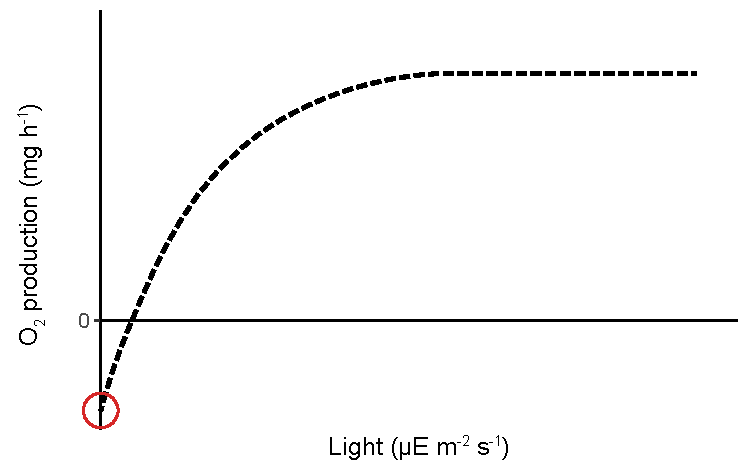
\includegraphics{../_chapter_materials/light_response_curve.pdf}
\caption{A photosynthesis light-response curve illustrates that as light
intensity increases, dissolved oxygen (DO) production eventually becomes
saturated. In the dark, photosynthesis shuts off, and respiration causes
the rate of DO production to fall below 0 (red circle on the y-axis).}
\end{figure}

\hypertarget{methods}{%
\subsection{Methods}\label{methods}}

\begin{enumerate}
\def\labelenumi{\arabic{enumi}.}
\tightlist
\item
  Each group will be responsible for \textbf{one} of the two species.
  Fill 9 BOD bottles with photosynthesis solution (fill to brim - the
  idea with BOD bottles is for the glass stopper to push any excess
  water out of the seal the stopper creates).
\item
  Carefully transfer a representative sample of your organism into 8 of
  the BOD bottles. Add a small stir bar to each bottle, and place the
  glass stopper and plastic cap on the bottle to seal. Use the DO probe
  to measure oxygen concentration in the remaining bottle (your control
  bottle).
\item
  You will have 4 replicates for the dark treatment, and 4 for the
  light. Wrap the dark treatment bottles in aluminum foil, and place the
  light treatment bottles under the light source.
  \underline{Record the intial times for these samples}.
\item
  While you wait (at least 1.5 hours)\ldots{}

  \begin{itemize}
  \tightlist
  \item
    Observe samples of these organisms under a dissecting/compound
    microscope and note differences in morphology. Note differences in
    the proportion of support tissues (i.e.~stems) vs.~photosynthetic
    tissues for each organism.
  \end{itemize}
\item
  After at least 1.5 hours, measure DO concentrations in the light
  bottles. Make sure to record the end time each time you take a DO
  measurement.
\item
  After 2 hours, measure the DO concentrations in the dark bottles. Make
  sure to record the end time each time you take a DO measurement.
\item
  Carefully empty the BOD bottle into a fine-mesh sieve to separate the
  sample from the photosynthesis solution. Collect/scrape the sample
  into a labeled aluminum drying tin, and place tins into a drying oven
  for 24 hrs at 105\textdegree{}C.
\end{enumerate}

\hypertarget{data-analysis}{%
\section{Data analysis}\label{data-analysis}}

You can directly determine P\textsubscript{net} (from the light
treatment bottles) and R (from the dark treatment bottles) by
calculating the change (\textDelta) in dissolved oxygen (DO)
concentrations:

\begin{equation}
\Delta{}DO = DO_{final} - DO_{initial}
(\#eq:delta)
\end{equation}

You also recorded the elapsed incubation time(\textDelta{}h), the volume
of the BOD bottles (0.330 L), and the mass of the sample (in dry weight,
g). Using equation @ref(eq:photosynthesis), after getting \textDelta{}DO
normalized to volume (L) and dry weight (g), you can then calculate
P\textsubscript{gross}, or the total oxygen produced by photosynthesis
per unit biomass.

For the 1\textsuperscript{st}, and 2\textsuperscript{nd} questions, a
two-sample t-test comparing the rates of each process
(P\textsubscript{gross} and R) will tell you if there are significant
differences between each organism. Bar-graphs (with error-bars display
the stardard error of the mean) are a good way of displaying this data
visually.

The 3\textsuperscript{rd} question requires you to construct a simple
\textbf{model}. A model is a way to represent a natural process using
mathematics. Some models are simple (like the one you will construct),
and some are incredibly complex. What assumptions can you make to tackle
question 3? If we assume that these organisms respire for 24 hours a
day, and only photosynthesize when the sun is out (10 hours a day), we
can use these values as a foundation for our model (Fig.
@ref(fig:photo-model)). While this makes the maths significantly easier,
what are the limitations of this assumption?

\begin{figure}
\centering
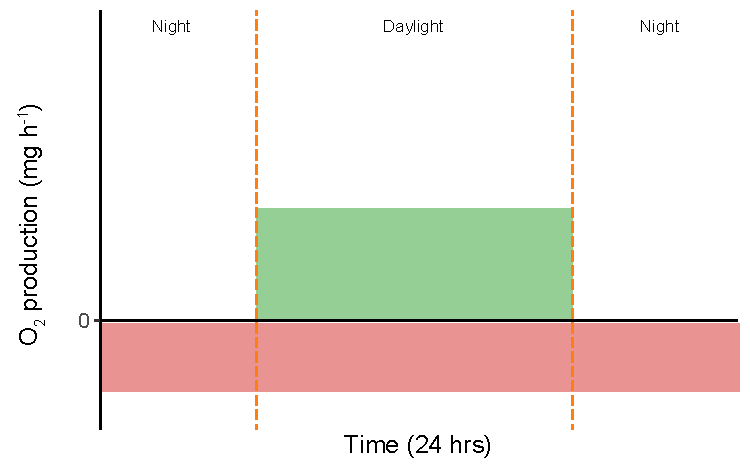
\includegraphics{../_chapter_materials/photo_model.pdf}
\caption{A photosynthesis light-response curve illustrates that as light
intensity increases, dissolved oxygen (DO) production eventually becomes
saturated. In the dark, photosynthesis shuts off, and respiration causes
the rate of DO production to fall below 0 (red circle on the y-axis).}
\end{figure}

There are no associated statistical tests for question 3, since you
should calculate daily values using mean P\textsubscript{gross} and mean
R (no replicate values for this question). You can present the results
of your model in the text of your results section.

\pagebreak

\hypertarget{lab-report-specifics}{%
\subsection{Lab report specifics}\label{lab-report-specifics}}

\begin{enumerate}
\def\labelenumi{\arabic{enumi}.}
\tightlist
\item
  Introduction

  \begin{itemize}
  \tightlist
  \item
    Importance of photosynthesis
  \item
    Morphological adaptations of aquatic photosynthesizers
  \item
    Objectives
  \item
    Hypotheses
  \end{itemize}
\item
  Methods

  \begin{itemize}
  \tightlist
  \item
    Oxygen change method (light/dark treatments)
  \item
    Experimental design
  \item
    Calculations / statistics / model explanation
  \end{itemize}
\item
  Results

  \begin{itemize}
  \tightlist
  \item
    Results/graphs/statistics for questions 1 and 2
  \item
    Results for question 3
  \end{itemize}
\item
  Discussion

  \begin{itemize}
  \tightlist
  \item
    Hypotheses rejected/supported?
  \item
    Provide a coherent explanation for the patterns you see in the
    photosynthesis and respiration data (use your observations of
    morphology and the information you covered in your introduction to
    tie everything together)
  \end{itemize}
\end{enumerate}

\pagebreak

\renewcommand{\arraystretch}{2}

\begin{landscape}\begin{table}[t]

\caption{\label{tab:unnamed-chunk-1}Datasheet for BOD experiment.}
\centering
\resizebox{\linewidth}{!}{
\fontsize{8}{10}\selectfont
\begin{tabular}{>{\raggedright\arraybackslash}p{1cm}l>{\raggedright\arraybackslash}p{1cm}>{\raggedright\arraybackslash}p{1cm}>{\raggedright\arraybackslash}p{1cm}>{\raggedright\arraybackslash}p{1cm}>{\raggedright\arraybackslash}p{1cm}>{\raggedright\arraybackslash}p{1cm}>{\raggedright\arraybackslash}p{1cm}>{\raggedright\arraybackslash}p{1cm}>{\raggedright\arraybackslash}p{1cm}>{\raggedright\arraybackslash}p{1cm}}
\toprule
BOD No. & Organism & Initial time (dark, hh:mm) & Initial DO (dark, mg/L) & Final time (dark, hh:mm) & Final DO (dark, mg/L) & Initial time (light, hh:mm) & Initial DO (light, mg/L) & Final time (light, hh:mm) & Final DO (light, mg/L) & Dish ID & Weight (g)\\
\midrule
\rowcolor{gray!6}   & Algae &  &  &  &  &  &  &  &  &  \vphantom{5} & \\
 & Algae &  &  &  &  &  &  &  &  &  \vphantom{4} & \\
\rowcolor{gray!6}   & Algae &  &  &  &  &  &  &  &  &  \vphantom{3} & \\
 & Algae &  &  &  &  &  &  &  &  &  \vphantom{2} & \\
\rowcolor{gray!6}   & Algae &  &  &  &  &  &  &  &  &  \vphantom{1} & \\
 & Algae &  &  &  &  &  &  &  &  &  & \\
\rowcolor{gray!6}   & Macrophyte &  &  &  &  &  &  &  &  &  \vphantom{5} & \\
 & Macrophyte &  &  &  &  &  &  &  &  &  \vphantom{4} & \\
\rowcolor{gray!6}   & Macrophyte &  &  &  &  &  &  &  &  &  \vphantom{3} & \\
 & Macrophyte &  &  &  &  &  &  &  &  &  \vphantom{2} & \\
\rowcolor{gray!6}   & Macrophyte &  &  &  &  &  &  &  &  &  \vphantom{1} & \\
 & Macrophyte &  &  &  &  &  &  &  &  &  & \\
\bottomrule
\end{tabular}}
\end{table}
\end{landscape}

\begin{landscape}\begin{table}[t]

\caption{\label{tab:unnamed-chunk-2}Calculation sheet for BOD experiment.}
\centering
\resizebox{\linewidth}{!}{
\fontsize{8}{10}\selectfont
\begin{tabular}{ll>{\raggedright\arraybackslash}p{2cm}>{\raggedright\arraybackslash}p{2cm}>{\raggedright\arraybackslash}p{2cm}>{\raggedright\arraybackslash}p{2cm}>{\raggedright\arraybackslash}p{2cm}>{\raggedright\arraybackslash}p{2cm}}
\toprule
BOD No. & Organism & Elapsed time (h) & Delta DO (mg/L) & Delta DO (mg) & Net photosynthesis (mg/(g*h)) & Respiration (mg/(g*h)) & Gross photosynthesis (mg/(g*h)\\
\midrule
\rowcolor{gray!6}   & Algae &  &  &  &  &  \vphantom{5} & \\
 & Algae &  &  &  &  &  \vphantom{4} & \\
\rowcolor{gray!6}   & Algae &  &  &  &  &  \vphantom{3} & \\
 & Algae &  &  &  &  &  \vphantom{2} & \\
\rowcolor{gray!6}   & Algae &  &  &  &  &  \vphantom{1} & \\
 & Algae &  &  &  &  &  & \\
\rowcolor{gray!6}   & Macrophyte &  &  &  &  &  \vphantom{5} & \\
 & Macrophyte &  &  &  &  &  \vphantom{4} & \\
\rowcolor{gray!6}   & Macrophyte &  &  &  &  &  \vphantom{3} & \\
 & Macrophyte &  &  &  &  &  \vphantom{2} & \\
\rowcolor{gray!6}   & Macrophyte &  &  &  &  &  \vphantom{1} & \\
 & Macrophyte &  &  &  &  &  & \\
\bottomrule
\end{tabular}}
\end{table}
\end{landscape}




\newpage
\singlespacing 
\end{document}
